\documentclass[11pt, a4paper, titlepage, oneside]{article}

\usepackage[T1]{fontenc}
\usepackage[ngerman]{babel}

\usepackage[left=2cm, right=2cm, top=2cm, bottom=2.25cm, includeheadfoot]{geometry}
\usepackage[labelfont=bf, textfont=it]{caption}
\usepackage{setspace}
\usepackage{tabularx}
\usepackage{colortbl}
\usepackage{fancyhdr}
\usepackage[stable]{footmisc}
\usepackage{listings}
\usepackage{xcolor}
\usepackage{fontspec}
\usepackage{pstricks}
\usepackage{wallpaper}

\linespread{1.25}

\newcommand{\heading}{SortSimulation}
\newcommand{\subheading}{Dokumentation}
\newcommand{\copyrightNotice}{Copyright \textcopyright{} 2008--2013 Peter Folta. Alle Rechte vorbehalten.}
\newcommand{\URL}{\href{http://www.peterfolta.net/software/sortsimulation}{http://www.peterfolta.net/software/sortsimulation}}
\newcommand{\version}{2.0.0}

\definecolor{pfColor1}{HTML}{62bd19}
\definecolor{pfColor2}{HTML}{339530}
\definecolor{pfColor3}{HTML}{bce18d}
\definecolor{pfColor4}{HTML}{00625a}

\usepackage[
	pdftitle = {SortSimulation},
	pdfsubject = {Dokumentation},
	pdfauthor = {Peter\ {}Folta},
	pdfkeywords = {},
	pdfcreator = {},
	pdfproducer = {},
	colorlinks = true,
	linkcolor = black,
	anchorcolor = black,
	citecolor = black,
	filecolor = black,
	menucolor = black,
	urlcolor = pfColor2]{hyperref}
	
\renewcommand{\lstlistingname}{Listing}
\renewcommand{\lstlistlistingname}{Listings}
\lstset{
	language			= java,
	sensitive			= false,
	basicstyle			= \footnotesize\ttfamily,
	commentstyle		= \itshape\color{comments},
	keywordstyle		= \bfseries\color{pfColor2},
	showstringspaces	= false,
	tabsize				= 4,
	numbers				= left,
	captionpos			= b,
	xleftmargin			= 3 em
}

% Header
\fancypagestyle{plain}{
\lhead{\heading{} -- \textit{\subheading}}
\chead{}
\rhead{\thepage}
\lfoot{}
\cfoot{\vspace{0.25cm}\psset{xunit=.25pt,yunit=.25pt,runit=.25pt}
\begin{pspicture}(447.45883179,69.47525024)
{
\newrgbcolor{curcolor}{0 0 0}
\pscustom[linestyle=none,fillstyle=solid,fillcolor=curcolor]
{
\newpath
\moveto(102.43471,34.20263024)
\curveto(103.13871,34.07463024)(103.20271,34.07463024)(103.39471,34.01063024)
\curveto(104.93071,33.81863024)(105.25071,33.75463024)(106.14671,33.75463024)
\curveto(114.4027,33.75463024)(120.54671,39.57863024)(120.54671,47.32263024)
\curveto(120.54671,53.72262024)(116.5147,56.92263024)(108.45071,56.92263024)
\lineto(107.68271,56.92263024)
\curveto(100.70672,56.79463024)(96.80271,56.73063024)(96.09871,56.73063024)
\curveto(94.75471,56.73063024)(94.7547,56.73063024)(85.02671,56.92263024)
\lineto(85.02671,54.55463024)
\lineto(87.39471,54.36263024)
\curveto(90.27471,54.10663024)(90.46671,53.72262024)(90.46671,48.09063024)
\lineto(90.46671,21.97863024)
\curveto(90.46671,16.28263024)(90.40271,16.15463024)(87.39471,15.89863024)
\lineto(85.02671,15.70663024)
\lineto(85.02671,13.14663024)
\curveto(92.7707,13.33863024)(92.77071,13.33863024)(95.01071,13.33863024)
\curveto(96.99471,13.33863024)(96.99472,13.33863024)(105.57071,13.14663024)
\lineto(105.57071,15.70663024)
\lineto(102.56271,15.89863024)
\curveto(99.61872,16.09063024)(99.49071,16.34663024)(99.49071,21.97863024)
\lineto(99.49071,53.14663024)
\curveto(100.45071,53.53063024)(101.60271,53.72263024)(103.33071,53.72263024)
\curveto(108.64271,53.72263024)(111.33071,50.84262024)(111.33071,45.14663024)
\curveto(111.33071,40.02663024)(108.77071,36.69863024)(104.73871,36.69863024)
\curveto(104.22671,36.69863024)(104.16271,36.69863024)(102.49871,37.01863024)
\curveto(102.43471,37.01863024)(102.24271,37.01863024)(101.98671,37.08263024)
\lineto(101.34671,36.44263024)
\lineto(102.43471,34.20263024)
\moveto(134.90571,44.33863024)
\curveto(137.70571,44.48863024)(139.40572,44.53863024)(142.15571,44.53863024)
\curveto(144.85571,44.53863024)(147.00571,44.08863024)(147.05571,43.53863024)
\lineto(147.45571,39.78863024)
\lineto(149.25571,39.78863024)
\lineto(149.95571,46.88863024)
\lineto(149.65571,47.23863024)
\curveto(147.80571,47.38863024)(146.85571,47.43863024)(144.90571,47.43863024)
\curveto(143.75571,47.43863024)(142.25571,47.38863024)(139.50571,47.33863024)
\curveto(135.85572,47.23863024)(134.45571,47.23863024)(133.00571,47.23863024)
\curveto(131.25571,47.23863024)(129.10571,47.28863024)(123.60571,47.38863024)
\lineto(123.60571,45.53863024)
\lineto(125.45571,45.38863024)
\curveto(127.70571,45.18863024)(127.85571,44.88862024)(127.85571,40.48863024)
\lineto(127.85571,18.08863024)
\curveto(127.85571,16.38863024)(127.60571,15.63863024)(126.85571,15.23863024)
\lineto(125.25571,14.33863024)
\lineto(125.25571,13.18863024)
\curveto(130.20571,13.33863024)(130.20571,13.33863024)(131.35571,13.33863024)
\lineto(133.05571,13.33863024)
\curveto(138.10571,13.18863024)(140.10572,13.13863024)(142.65571,13.13863024)
\curveto(145.25571,13.13863024)(146.80572,13.18863024)(149.70571,13.33863024)
\lineto(149.95571,13.73863024)
\lineto(150.50571,21.63863024)
\lineto(148.55571,21.63863024)
\lineto(147.40571,16.93863024)
\curveto(147.40571,16.88863024)(147.35571,16.83863024)(147.25571,16.78863024)
\curveto(145.70571,16.28863024)(144.25571,16.08863024)(141.45571,16.08863024)
\curveto(139.40571,16.08863024)(137.45571,16.13863024)(134.90571,16.23863024)
\lineto(134.90571,29.58863024)
\curveto(136.30571,29.68863024)(137.15571,29.73863024)(138.25571,29.73863024)
\lineto(141.55571,29.73863024)
\curveto(143.45571,29.73863024)(144.25571,29.18863024)(144.40571,27.88863024)
\lineto(144.70571,25.38863024)
\lineto(146.70571,25.38863024)
\lineto(146.55571,30.78863024)
\curveto(146.55571,31.33863024)(146.55571,31.38863024)(146.70571,36.13863024)
\lineto(144.70571,36.13863024)
\lineto(144.40571,33.28863024)
\curveto(144.30571,32.48863024)(143.65571,32.23863024)(141.55571,32.23863024)
\lineto(138.25571,32.23863024)
\curveto(136.60571,32.23863024)(135.90571,32.23863024)(134.90571,32.33863024)
\lineto(134.90571,44.33863024)
\moveto(172.42212,44.28863024)
\lineto(178.27212,44.28863024)
\curveto(180.37212,44.28863024)(180.92212,44.18863024)(181.37212,43.83863024)
\lineto(181.82212,42.63863024)
\lineto(182.07212,39.18863024)
\lineto(184.07212,39.18863024)
\curveto(184.17212,42.98862024)(184.32212,44.73863024)(184.72212,47.13863024)
\lineto(184.42212,47.38863024)
\curveto(170.62213,47.23863024)(170.62212,47.23863024)(168.92212,47.23863024)
\curveto(167.17212,47.23863024)(167.17211,47.23863024)(153.37212,47.38863024)
\lineto(153.07212,47.13863024)
\curveto(153.47212,44.73863024)(153.57212,42.98862024)(153.72212,39.18863024)
\lineto(155.72212,39.18863024)
\lineto(155.97212,42.63863024)
\curveto(155.97212,42.93863024)(156.22212,43.53863024)(156.37212,43.78863024)
\curveto(156.62212,44.13863024)(157.42212,44.28863024)(159.52212,44.28863024)
\lineto(165.37212,44.28863024)
\lineto(165.37212,20.08863024)
\curveto(165.37212,15.63863024)(165.32212,15.53863024)(162.97212,15.33863024)
\lineto(161.12212,15.18863024)
\lineto(161.12212,13.18863024)
\curveto(167.17211,13.33863024)(167.17212,13.33863024)(168.87212,13.33863024)
\curveto(170.57212,13.33863024)(170.62212,13.33863024)(176.67212,13.18863024)
\lineto(176.67212,15.18863024)
\lineto(174.82212,15.33863024)
\curveto(172.47212,15.53863024)(172.42212,15.63863024)(172.42212,20.08863024)
\lineto(172.42212,44.28863024)
\moveto(198.87056,44.33863024)
\curveto(201.67055,44.48863024)(203.37056,44.53863024)(206.12056,44.53863024)
\curveto(208.82055,44.53863024)(210.97056,44.08863024)(211.02056,43.53863024)
\lineto(211.42056,39.78863024)
\lineto(213.22056,39.78863024)
\lineto(213.92056,46.88863024)
\lineto(213.62056,47.23863024)
\curveto(211.77056,47.38863024)(210.82055,47.43863024)(208.87056,47.43863024)
\curveto(207.72056,47.43863024)(206.22055,47.38863024)(203.47056,47.33863024)
\curveto(199.82056,47.23863024)(198.42055,47.23863024)(196.97056,47.23863024)
\curveto(195.22056,47.23863024)(193.07055,47.28863024)(187.57056,47.38863024)
\lineto(187.57056,45.53863024)
\lineto(189.42056,45.38863024)
\curveto(191.67055,45.18863024)(191.82056,44.88862024)(191.82056,40.48863024)
\lineto(191.82056,18.08863024)
\curveto(191.82056,16.38863024)(191.57056,15.63863024)(190.82056,15.23863024)
\lineto(189.22056,14.33863024)
\lineto(189.22056,13.18863024)
\curveto(194.17055,13.33863024)(194.17056,13.33863024)(195.32056,13.33863024)
\lineto(197.02056,13.33863024)
\curveto(202.07055,13.18863024)(204.07056,13.13863024)(206.62056,13.13863024)
\curveto(209.22055,13.13863024)(210.77056,13.18863024)(213.67056,13.33863024)
\lineto(213.92056,13.73863024)
\lineto(214.47056,21.63863024)
\lineto(212.52056,21.63863024)
\lineto(211.37056,16.93863024)
\curveto(211.37056,16.88863024)(211.32056,16.83863024)(211.22056,16.78863024)
\curveto(209.67056,16.28863024)(208.22055,16.08863024)(205.42056,16.08863024)
\curveto(203.37056,16.08863024)(201.42055,16.13863024)(198.87056,16.23863024)
\lineto(198.87056,29.58863024)
\curveto(200.27055,29.68863024)(201.12056,29.73863024)(202.22056,29.73863024)
\lineto(205.52056,29.73863024)
\curveto(207.42055,29.73863024)(208.22056,29.18863024)(208.37056,27.88863024)
\lineto(208.67056,25.38863024)
\lineto(210.67056,25.38863024)
\lineto(210.52056,30.78863024)
\curveto(210.52056,31.33863024)(210.52056,31.38863024)(210.67056,36.13863024)
\lineto(208.67056,36.13863024)
\lineto(208.37056,33.28863024)
\curveto(208.27056,32.48863024)(207.62055,32.23863024)(205.52056,32.23863024)
\lineto(202.22056,32.23863024)
\curveto(200.57056,32.23863024)(199.87056,32.23863024)(198.87056,32.33863024)
\lineto(198.87056,44.33863024)
\moveto(239.03696,31.13863024)
\curveto(241.83696,32.28863024)(243.03696,33.03863024)(244.33696,34.53863024)
\curveto(245.78696,36.08862024)(246.48696,37.93863024)(246.48696,40.03863024)
\curveto(246.48696,44.88862024)(243.28696,47.38863024)(236.98696,47.38863024)
\curveto(236.43696,47.38863024)(235.23696,47.38863024)(233.53696,47.33863024)
\curveto(232.23696,47.28863024)(228.13696,47.23863024)(227.03696,47.23863024)
\curveto(225.63696,47.23863024)(225.63696,47.23863024)(218.13696,47.38863024)
\lineto(218.13696,45.53863024)
\lineto(219.98696,45.38863024)
\curveto(222.23696,45.18863024)(222.38696,44.88862024)(222.38696,40.48863024)
\lineto(222.38696,20.08863024)
\curveto(222.38696,15.63863024)(222.33696,15.53863024)(219.98696,15.33863024)
\lineto(218.13696,15.18863024)
\lineto(218.13696,13.18863024)
\curveto(224.18696,13.33863024)(224.18696,13.33863024)(225.88696,13.33863024)
\curveto(227.58696,13.33863024)(227.63697,13.33863024)(233.68696,13.18863024)
\lineto(233.68696,15.18863024)
\lineto(231.83696,15.33863024)
\curveto(229.48696,15.53863024)(229.43696,15.63863024)(229.43696,20.08863024)
\lineto(229.43696,44.43863024)
\curveto(230.13696,44.73863024)(231.08696,44.88863024)(232.38696,44.88863024)
\curveto(236.83696,44.88863024)(239.38696,42.53862024)(239.38696,38.48863024)
\curveto(239.38696,35.83863024)(238.13696,33.58863024)(236.08696,32.38863024)
\curveto(234.83696,31.63863024)(233.58696,31.38863024)(231.38696,31.43863024)
\lineto(231.03696,30.53863024)
\lineto(242.23696,13.18863024)
\lineto(246.73696,13.33863024)
\curveto(249.28696,13.28863024)(249.73696,13.28863024)(251.58696,13.18863024)
\lineto(251.58696,15.18863024)
\curveto(249.78696,15.53863024)(249.28696,15.83863024)(248.08696,17.43863024)
\lineto(239.03696,31.13863024)
\moveto(284.57578,53.01863024)
\curveto(287.71177,53.14663024)(289.82378,53.21063024)(291.99978,53.21063024)
\curveto(296.28777,53.21063024)(299.03978,52.76263024)(299.10378,51.99463024)
\lineto(299.61578,47.19463024)
\lineto(301.91978,47.19463024)
\lineto(302.81578,56.28263024)
\lineto(302.43178,56.73063024)
\curveto(299.99978,56.92263024)(298.84777,56.98663024)(296.35178,56.98663024)
\curveto(294.87978,56.98663024)(292.44777,56.92263024)(287.32778,56.79463024)
\curveto(284.38378,56.73063024)(282.78377,56.73063024)(281.50378,56.73063024)
\curveto(279.64778,56.73063024)(279.64777,56.73063024)(270.11178,56.92263024)
\lineto(270.11178,54.55463024)
\lineto(272.47978,54.36263024)
\curveto(275.35977,54.10663024)(275.55178,53.72262024)(275.55178,48.09063024)
\lineto(275.55178,21.97863024)
\curveto(275.55178,16.28263024)(275.48777,16.15463024)(272.47978,15.89863024)
\lineto(270.11178,15.70663024)
\lineto(270.11178,13.14663024)
\curveto(277.85577,13.33863024)(277.85578,13.33863024)(280.03178,13.33863024)
\curveto(282.07977,13.33863024)(282.07978,13.33863024)(290.65578,13.14663024)
\lineto(290.65578,15.70663024)
\lineto(287.64778,15.89863024)
\curveto(284.70378,16.09063024)(284.57578,16.34663024)(284.57578,21.97863024)
\lineto(284.57578,33.94663024)
\curveto(286.36777,34.07463024)(287.45578,34.13863024)(288.86378,34.13863024)
\lineto(292.12778,34.13863024)
\curveto(294.55977,34.13863024)(295.58378,33.43462024)(295.77578,31.77063024)
\lineto(296.15978,28.57063024)
\lineto(298.71978,28.57063024)
\lineto(298.52778,35.48263024)
\curveto(298.52778,36.18663024)(298.52778,37.08263024)(298.71978,42.07463024)
\lineto(296.15978,42.07463024)
\lineto(295.77578,38.68263024)
\curveto(295.64778,37.65863024)(294.81577,37.33863024)(292.12778,37.33863024)
\lineto(288.86378,37.33863024)
\curveto(286.75178,37.33863024)(285.85577,37.33863024)(284.57578,37.46663024)
\lineto(284.57578,53.01863024)
\moveto(325.44478,48.08863024)
\curveto(313.34479,48.08863024)(306.29478,41.38862024)(306.29478,29.93863024)
\curveto(306.29478,18.83864024)(312.84479,12.48863024)(324.29478,12.48863024)
\curveto(336.24476,12.48863024)(343.29478,19.23864024)(343.29478,30.63863024)
\curveto(343.29478,41.63862024)(336.74476,48.08863024)(325.44478,48.08863024)
\moveto(324.99478,45.28863024)
\curveto(327.64477,45.28863024)(329.74478,44.43862024)(331.49478,42.73863024)
\curveto(334.24477,40.03863024)(335.79478,35.23862024)(335.79478,29.58863024)
\curveto(335.79478,20.18864024)(331.94477,15.28863024)(324.64478,15.28863024)
\curveto(321.89478,15.28863024)(319.84477,16.08863024)(318.04478,17.88863024)
\curveto(315.34478,20.53862024)(313.79478,25.33863024)(313.79478,31.08863024)
\curveto(313.79478,36.18862024)(315.04478,40.18863024)(317.29478,42.43863024)
\curveto(319.24477,44.33862024)(321.84478,45.28863024)(324.99478,45.28863024)
\moveto(358.89399,40.48863024)
\curveto(358.89399,44.93862024)(358.944,45.03863024)(361.29399,45.23863024)
\lineto(363.14399,45.38863024)
\lineto(363.14399,47.38863024)
\curveto(357.044,47.23863024)(357.04399,47.23863024)(355.34399,47.23863024)
\curveto(353.644,47.23863024)(353.59399,47.23863024)(347.59399,47.38863024)
\lineto(347.59399,45.38863024)
\lineto(349.44399,45.23863024)
\curveto(351.79399,45.03863024)(351.84399,44.93862024)(351.84399,40.48863024)
\lineto(351.84399,18.08863024)
\curveto(351.84399,16.38863024)(351.59399,15.63863024)(350.84399,15.23863024)
\lineto(349.24399,14.33863024)
\lineto(349.24399,13.18863024)
\curveto(354.19399,13.33863024)(354.19399,13.33863024)(355.34399,13.33863024)
\lineto(357.04399,13.33863024)
\curveto(362.09399,13.18863024)(364.094,13.13863024)(366.64399,13.13863024)
\curveto(369.24399,13.13863024)(370.794,13.18863024)(373.69399,13.33863024)
\lineto(373.94399,13.73863024)
\lineto(374.49399,22.03863024)
\lineto(372.54399,22.03863024)
\lineto(371.39399,16.93863024)
\curveto(371.29399,16.48863024)(368.54399,16.08863024)(365.44399,16.08863024)
\curveto(363.344,16.08863024)(361.49399,16.13863024)(358.89399,16.23863024)
\lineto(358.89399,40.48863024)
\moveto(396.4104,44.28863024)
\lineto(402.2604,44.28863024)
\curveto(404.3604,44.28863024)(404.9104,44.18863024)(405.3604,43.83863024)
\lineto(405.8104,42.63863024)
\lineto(406.0604,39.18863024)
\lineto(408.0604,39.18863024)
\curveto(408.1604,42.98862024)(408.3104,44.73863024)(408.7104,47.13863024)
\lineto(408.4104,47.38863024)
\curveto(394.61041,47.23863024)(394.6104,47.23863024)(392.9104,47.23863024)
\curveto(391.1604,47.23863024)(391.16039,47.23863024)(377.3604,47.38863024)
\lineto(377.0604,47.13863024)
\curveto(377.4604,44.73863024)(377.5604,42.98862024)(377.7104,39.18863024)
\lineto(379.7104,39.18863024)
\lineto(379.9604,42.63863024)
\curveto(379.9604,42.93863024)(380.2104,43.53863024)(380.3604,43.78863024)
\curveto(380.6104,44.13863024)(381.4104,44.28863024)(383.5104,44.28863024)
\lineto(389.3604,44.28863024)
\lineto(389.3604,20.08863024)
\curveto(389.3604,15.63863024)(389.3104,15.53863024)(386.9604,15.33863024)
\lineto(385.1104,15.18863024)
\lineto(385.1104,13.18863024)
\curveto(391.16039,13.33863024)(391.1604,13.33863024)(392.8604,13.33863024)
\curveto(394.5604,13.33863024)(394.61041,13.33863024)(400.6604,13.18863024)
\lineto(400.6604,15.18863024)
\lineto(398.8104,15.33863024)
\curveto(396.4604,15.53863024)(396.4104,15.63863024)(396.4104,20.08863024)
\lineto(396.4104,44.28863024)
\moveto(433.05884,23.63863024)
\lineto(435.30884,17.93863024)
\curveto(435.50884,17.43863024)(435.60884,16.93863024)(435.60884,16.53863024)
\curveto(435.60884,15.78863024)(435.15884,15.23863024)(434.60884,15.18863024)
\lineto(431.95884,15.03863024)
\lineto(431.95884,13.18863024)
\curveto(438.95883,13.33863024)(438.95884,13.33863024)(439.55884,13.33863024)
\curveto(440.10884,13.33863024)(440.10884,13.33863024)(447.45884,13.18863024)
\lineto(447.45884,15.03863024)
\lineto(446.25884,15.18863024)
\curveto(444.85884,15.38863024)(444.15884,15.93863024)(443.50884,17.38863024)
\lineto(430.55884,47.63863024)
\lineto(427.00884,47.63863024)
\lineto(425.60884,43.88863024)
\curveto(424.90884,41.93863024)(424.40884,40.63863024)(424.15884,40.08863024)
\lineto(415.10884,18.18863024)
\curveto(414.25884,16.23863024)(413.40884,15.28863024)(412.30884,15.18863024)
\lineto(410.80884,15.03863024)
\lineto(410.80884,13.18863024)
\curveto(412.10884,13.23863024)(413.25884,13.23863024)(413.65884,13.28863024)
\curveto(415.05884,13.33863024)(416.00884,13.33863024)(416.45884,13.33863024)
\curveto(416.90884,13.33863024)(417.85884,13.33863024)(419.25884,13.28863024)
\curveto(419.70884,13.23863024)(420.75884,13.23863024)(422.10884,13.18863024)
\lineto(422.10884,15.03863024)
\lineto(419.60884,15.18863024)
\curveto(418.75884,15.23863024)(418.15884,15.93863024)(418.15884,16.78863024)
\curveto(418.15884,17.13863024)(418.25884,17.63863024)(418.40884,18.03863024)
\lineto(420.50884,23.63863024)
\lineto(433.05884,23.63863024)
\moveto(426.70884,39.13863024)
\lineto(431.90884,26.43863024)
\lineto(421.70884,26.43863024)
\lineto(426.70884,39.13863024)
}
}
{
\newrgbcolor{curcolor}{0 0 0}
\pscustom[linewidth=4.5,linecolor=curcolor]
{
\newpath
\moveto(67.22525,34.73763024)
\curveto(67.22525,16.79521024)(52.68005,2.25000024)(34.73763,2.25000024)
\curveto(16.79522,2.25000024)(2.25,16.79521024)(2.25,34.73763024)
\curveto(2.25,52.68005024)(16.79522,67.22525024)(34.73763,67.22525024)
\curveto(52.68005,67.22525024)(67.22525,52.68005024)(67.22525,34.73763024)
\closepath
}
}
{
\newrgbcolor{curcolor}{0 0 0}
\pscustom[linestyle=none,fillstyle=solid,fillcolor=curcolor]
{
\newpath
\moveto(22.70435,48.10520024)
\lineto(27.38056,48.10520024)
\curveto(30.4164,48.10516024)(33.01157,47.01976024)(35.16607,44.84899024)
\curveto(37.32052,42.69448024)(38.39776,40.09932024)(38.39779,37.06348024)
\lineto(38.39779,32.38728024)
\curveto(38.39776,29.35140024)(37.32052,26.75624024)(35.16607,24.60177024)
\curveto(33.01157,22.44728024)(30.4164,21.37004024)(27.38056,21.37005024)
\lineto(23.43884,21.37005024)
\lineto(19.5216,21.37005024)
\curveto(18.37906,21.37004024)(17.31815,21.59038024)(16.33884,22.03108024)
\lineto(16.33884,21.37005024)
\lineto(16.33884,12.67868024)
\curveto(16.33884,11.11179024)(15.56355,10.32833024)(14.01298,10.32833024)
\lineto(14.01298,10.32833024)
\curveto(12.44609,10.32833024)(11.66264,11.11179024)(11.66264,12.67868024)
\lineto(11.66264,24.87108024)
\lineto(11.66264,37.06348024)
\curveto(11.66264,40.09932024)(12.73988,42.69448024)(14.89436,44.84899024)
\curveto(17.06516,47.01976024)(19.66849,48.10516024)(22.70435,48.10520024)
\moveto(27.38056,26.04626024)
\curveto(29.12698,26.04624024)(30.62042,26.66646024)(31.8609,27.90694024)
\curveto(33.10134,29.14738024)(33.72157,30.64084024)(33.72159,32.38728024)
\lineto(33.72159,37.06348024)
\curveto(33.72157,38.80989024)(33.10134,40.30334024)(31.8609,41.54382024)
\curveto(30.62042,42.80057024)(29.12698,43.42896024)(27.38056,43.42900024)
\lineto(22.70435,43.42900024)
\curveto(20.94159,43.42896024)(19.43998,42.80057024)(18.19953,41.54382024)
\curveto(16.95907,40.30334024)(16.33884,38.80989024)(16.33884,37.06348024)
\lineto(16.33884,29.05763024)
\lineto(16.33884,29.05763024)
\curveto(16.3878,28.22520024)(16.71424,27.51520024)(17.31815,26.92763024)
\curveto(17.93838,26.34003024)(18.67286,26.04624024)(19.5216,26.04626024)
\curveto(20.82734,26.04624024)(22.13308,26.04624024)(23.43884,26.04626024)
\curveto(24.74457,26.04624024)(26.05848,26.04624024)(27.38056,26.04626024)
\moveto(47.62778,48.10520024)
\curveto(48.5418,48.10516024)(49.45582,48.10516024)(50.36985,48.10520024)
\curveto(51.28386,48.10516024)(52.20604,48.10516024)(53.1364,48.10520024)
\curveto(54.70328,48.10516024)(55.48673,47.32171024)(55.48674,45.75486024)
\lineto(55.48674,45.75486024)
\curveto(55.48673,44.20426024)(54.70328,43.42896024)(53.1364,43.42900024)
\curveto(52.20604,43.42896024)(51.28386,43.42896024)(50.36985,43.42900024)
\curveto(49.45582,43.42896024)(48.5418,43.42896024)(47.62778,43.42900024)
\curveto(46.77904,43.42896024)(46.04456,43.13517024)(45.42434,42.54762024)
\curveto(44.82042,41.96000024)(44.49399,41.25000024)(44.44503,40.41762024)
\lineto(44.44503,40.41762024)
\lineto(44.44503,23.69592024)
\curveto(44.44502,22.14532024)(43.66974,21.37004024)(42.11917,21.37005024)
\lineto(42.11917,21.37005024)
\curveto(40.55227,21.37004024)(39.76882,22.14532024)(39.76882,23.69592024)
\lineto(39.76882,35.88831024)
\lineto(39.76882,48.10520024)
\curveto(39.76882,51.14102024)(40.84606,53.73620024)(43.00055,55.89071024)
\curveto(45.17134,58.06146024)(47.77467,59.14687024)(50.81054,59.14692024)
\curveto(52.24685,59.14687024)(53.01397,59.14687024)(53.11192,59.14692024)
\curveto(53.22616,59.14687024)(54.01776,59.14687024)(55.48674,59.14692024)
\curveto(57.0373,59.14687024)(57.81258,58.36342024)(57.8126,56.79657024)
\lineto(57.8126,56.79657024)
\curveto(57.81258,55.22963024)(57.0373,54.44618024)(55.48674,54.44623024)
\curveto(54.01776,54.44618024)(53.22616,54.44618024)(53.11192,54.44623024)
\curveto(53.01397,54.44618024)(52.24685,54.44618024)(50.81054,54.44623024)
\curveto(49.04777,54.44618024)(47.54617,53.82595024)(46.30572,52.58554024)
\curveto(45.06525,51.34504024)(44.44502,49.85159024)(44.44503,48.10520024)
\lineto(44.44503,47.41968024)
\curveto(45.45697,47.87666024)(46.51789,48.10516024)(47.62778,48.10520024)
}
}
\end{pspicture}
}
\rfoot{}
\renewcommand{\headrulewidth}{0.5pt}
\renewcommand{\footrulewidth}{0.5pt}
}
\pagestyle{plain}

% Absatzeinrückung
\parindent 0pt

% Emphasize fett statt kursiv
\renewcommand{\emph}{\textbf}

\renewcommand\arraystretch{1.5}

\setmainfont[Ligatures=TeX]{Liberation Sans}
\setmonofont{Liberation Mono}

\begin{document}
	\ThisCenterWallPaper{1.0}{titlewallpaper.pdf}
	\pagenumbering{roman}
	
	\begin{titlepage}
		\begin{center}
			\vspace*{2.5cm}
			\Huge{\textbf{SortSimulation}}
			
			\vspace*{1.5cm}
			\LARGE{Dokumentation}
			
			\Large{-- Deutsch --}
			
			\vspace*{3.75cm}
			\Large{Peter Folta}
		\end{center}
		
		\vspace*{8cm}
		\noindent{}Version \version\newline{}
		Internet: \URL\newline{}
		\copyrightNotice
	\end{titlepage}
	
	\CenterWallPaper{1.0}{wallpaper.pdf}
	\setcounter{page}{2}
	
	\cleardoublepage{}
	\tableofcontents{}
	\newpage{}
	
	\pagenumbering{arabic}
	
	\section{Einführung}
	
	SortSimulation ist ein Java-Programm, das diverse Sortierverfahren visuell darstellt. Dies ermöglicht einerseits ein besseres Verständnis der Funktionsweise der verschiedenen Sortieralgorithmen und verdeutlicht andererseits die Laufzeitunterschiede, ohne dabei lediglich trockene Zahlen zu vergleichen.
	
	\begin{figure}[h]
		\centering
		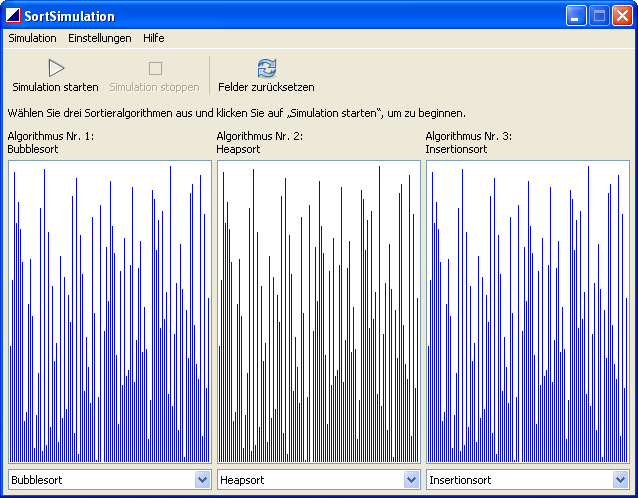
\includegraphics[scale=0.6]{images/image0.png}
		\caption{Das Hauptfenster von SortSimulation}
	\end{figure}
	
	Diese Dokumentation enthält eine kurze Einführung in die Bedienung von SortSimulation und stellt anschließend die unterstützten Sortierverfahren inklusive Implementierung in Java vor.
	
	\section{Bedienung}
	
	Die Bedienung von SortSimulation ist denkbar einfach: Direkt nach dem Programmstart sind die Sortierfelder bereits zufällig gefüllt. Dabei liegt in jedem der drei Felder die gleiche Ausgangssituation vor. Ebenfalls sind nach dem Programmstart drei verschiedene Sortierverfahren voreingestellt; dies ist an den Auswahlboxen unterhalb der Sortierfelder erkennbar.
	
	Um nun drei Sortieralgorithmen miteinander zu vergleichen, wählen Sie aus den Auswahlboxen die entsprechenden Verfahren aus. Die Simulation startet, sobald Sie auf die Schaltfläche \emph{Simulation starten} in der Toolbar klicken, den entsprechenden Eintrag im Menü \emph{Simulation} auswählen oder die Eingabetaste drücken. Möchten Sie eine laufende Simulation abbrechen, genügt ein Druck auf die Escape-Taste oder ein Klick auf die Schaltfläche \emph{Simulation stoppen}. Um nach einer abgeschlossenen oder abgebrochenen Simulation wieder unsortierte Felder zu erhalten, klicken Sie auf die Schaltfläche \emph{Felder zurücksetzen} oder drücken Sie \texttt{Strg+N}.
	
	SortSimulation bietet einige Einstellungen, mit denen Sie die Simulation anpassen können. Auf diese Einstellungen wird im folgenden Abschnitt ausführlich eingegangen.
	
	\subsection{Einstellungen}
	
	Ihnen stehen in SortSimulation diverse Einstellungen zur Verfügung, mit denen Sie die Sortier-Simulationen ihren Wünschen entsprechend anpassen können. Diese Ein\-{}stellungs\-{}mög\-{}lich\-{}kei\-{}ten finden Sie im Menü \emph{Einstellungen}:
	
	\begin{figure}[h]
		\centering
		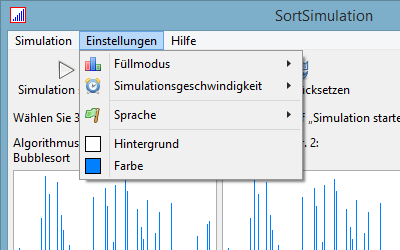
\includegraphics[scale=0.6]{images/image1.png}
		\caption{Menü "`Einstellungen"'}
	\end{figure}
	
	Mithilfe der Option \emph{Füllmodus} können Sie festlegen, auf welche Weise die Sortierfelder gefüllt werden sollen, wenn die Aktion \emph{Felder zurücksetzen} ausgeführt wird. Dabei stehen zwei Modi zur Verfügung: Zufällig (voreingestellt; \texttt{Strg+R}) und Invers (\texttt{Strg+I}). Im Modus \emph{Zufällig} werden die Elemente bei jeder Neufüllung der Felder zufällig angeordnet. Damit lassen sich die unterschiedlichen Sortierverfahren auf realistische Weise mit völlig unsortierten Daten ausprobieren.
	
	Im Modus \emph{Invers} hingegen werden die Felder bereits sortiert gefüllt~-- allerdings umgekehrt (absteigend statt aufsteigend). Mit dieser Einstellung lässt sich beobachten, wie effizient die Sortierverfahren umgekehrt geordnete Folgen sortieren.
	
	Das Untermenü \emph{Simulationsgeschwindigkeit} ermöglicht es Ihnen, die Geschwindigkeit der Simulation anzupassen. Sie haben dabei die Wahl zwischen fünf Stufen. Während Algorithmen wie etwa Bubblesort sehr langsam sind und sich dort eine hohe Simulationsgeschwindigkeit anbietet, lohnt es sich, beispielsweise Quicksort in einer langsamen Stufe zu beobachten, um die Vorgehensweise dieses Verfahrens besser verstehen zu können. Die einzelnen Geschwindigkeitsstufen lassen sich auch über die Tastatur mithilfe der Tastenkombinationen \texttt{Strg+Umschalt+(1-5)} erreichen.
	
	SortSimulation schreibt oder verändert keine Dateien auf Ihrem Computer, das Programm startet deshalb jedes Mal mit der englischen Benutzeroberfläche. Sie können die Sprache im Menü \emph{Sprache} (engl. \emph{Settings} > \emph{Language}) verändern.
	
	Im letzten Untermenü \emph{Farbe} kann die Farbe der Balken eingestellt werden. Stan\-{}dard\-{}mäßig ist Blau eingestellt, Sie haben jedoch die Wahl zwischen acht verschiedenen Farben.
	
	\section{Sortierverfahren}
	
	\subsection{Bubblesort}
	
	Bubblesort ist ein einfacher Sortieralgorithmus, der Elemente durch \emph{schrittweises Vergleichen} sortiert. Da Bubblesort nicht effizient ist, wird der Algorithmus häufig zur Demonstration eines schlechten Sortierverfahrens verwendet.
	
	\subsubsection{Idee von Bubblesort}
	
	Bubblesort vergleicht zwei benachbarte Elemente und vertauscht diese, wenn sie nicht in der richtigen Reihenfolge stehen. Dieser Vorgang wird solange wiederholt, bis alle Elemente an der richtigen Stelle stehen und damit sortiert sind.
	
	\subsubsection{Implementierung in Java}
	
	\lstinputlisting[caption={Implementierung von Bubblesort}, label=lst:bubblesort, captionpos=b]{../Listings/Bubblesort.java}
	
	\subsection{Heapsort}
	
	Heapsort ist ein schnelles Sortierverfahren, das 1964 von \emph{Robert W. Floyd} und \emph{J.\,W.\,J. Williams} entwickelt wurde. Heapsort ist eine Verbesserung des Sortieralgorithmus \emph{Selectionsort}.
	
	\subsubsection{Idee von Heapsort}
	
	Heapsort verwendet zur Sortierung eine besondere Datenstruktur: den \emph{Heap}. Diese Datenstruktur basiert auf einem (fast) vollständigen \emph{binären Baum}. Ein binärer Baum ist (fast) vollständig, wenn alle Ebenen, außer möglicherweise der letzten, vollständig sind.
	
	Wenn die zu sortierende Folge als Heap vorliegt, kann das größte Element der \emph{Wurzel} des Baumes entnommen und ausgegeben werden. Um an das nächstgrößte Element zu gelangen, muss der Heap zunächst \emph{neu angeordnet} werden.
	
	\subsubsection{Implementierung in Java}
	
	\lstinputlisting[caption={Implementierung von Heapsort}, label=lst:heapsort, captionpos=b]{../Listings/Heapsort.java}
	
	\subsection{Insertionsort}
	
	Insertionsort ist ein einfaches Sortierverfahren. Es ist nicht so effizient, wie andere komplexere Algorithmen, dafür aber \emph{einfach zu implementieren} und benötigt nur eine kurze Laufzeit bei sehr kleinen oder bereits vorsortierten Datenmengen.
	
	\subsubsection{Idee von Insertionsort}
	
	Insertionsort entnimmt der unsortierten Menge ein Element und fügt es an der richtigen Stelle in der Ausgabefolge ein. Ist die Folge noch leer, wird das Element an die erste Position eingefügt.
	
	Insertionsort ist ineffizient, da bei diesem Sortierverfahren Elemente oft über weite Strecken verschoben werden müssen.
	
	\subsubsection{Implementierung in Java}
	
	\lstinputlisting[caption={Implementierung von Insertionsort}, label=lst:insertionsort, captionpos=b]{../Listings/Insertionsort.java}
	
	\subsection{Mergesort}
	
	Mergesort ist ein rekursiver und stabiler Sortieralgorithmus, welcher wie \emph{Quicksort} auf dem \emph{Divide-and-Conquer-Prinzip} basiert. Mergesort wurde 1945 von John von Neumann vorgestellt.
	
	\subsubsection{Idee von Mergesort}
	
	Mergesort zerlegt die zu sortierende Folge in mehrere kleine Folgen, die, jede für sich, sortiert werden. Anschließend werden die sortierten, kleinen Folgen im Reißverschlussverfahren wieder zu einer großen Folge zusammengesetzt, bis alle Elemente sortiert sind.
	
	\subsubsection{Implementierung in Java}
	
	\lstinputlisting[caption={Implementierung von Mergesort}, label=lst:mergesort, captionpos=b]{../Listings/Mergesort.java}
	
	\subsection{Quicksort}
	
	Quicksort ist eines der \emph{schnellsten Sortierverfahren} und basiert auf dem \emph{Divide-and-Conquer-Prinzip}. Der rekursive Quicksort-Algorithmus wurde in seiner ursprünglichen Fassung im Jahre 1960 von \emph{C. Antony R. Hoare} entwickelt.
	
	\subsubsection{Idee von Quicksort}
	
	Die zu sortierende Folge wird zunächst so in zwei Teilstücke zerlegt, dass alle Elemente im ersten Teilstück kleiner oder gleich allen Elementen im zweiten Teilstück sind (\emph{divide}). Anschließend werden die beiden Teilstücke unabhängig voneinander rekursiv nach dem gleichen Verfahren sortiert (\emph{conquer}). Im letzten Schritt ergeben die zusammengesetzten Teilstücke die sortierte Folge (\emph{combine}).
	
	Die Aufteilung wird mit Hilfe eines \emph{Pivotelementes} realisiert, das im ersten Schritt aus der Folge gewählt wird. Alle Elemente der Folge, die \emph{kleiner} als das Pivotelement sind, kommen in das erste Teilstück. Alle Elemente, die \emph{größer} als das Pivotelement sind, kommen in das zweite Teilstück. Bei Elementen, die genauso groß wie das Pivotelement sind, spielt es keine Rolle, in welches Teilstück sie kommen.
	
	\subsubsection{Implementierung in Java}
	
	\lstinputlisting[caption={Implementierung von Quicksort}, label=lst:quicksort, captionpos=b]{../Listings/Quicksort.java}
	
	\subsection{Selectionsort}
	
	Selectionsort ist ein naiver Sortieralgorithmus, der in-place arbeitet. Er ist mit Insertionsort vergleichbar.
	
	\subsubsection{Idee von Selectionsort}
	
	Selectionsort teilt die zu sortierende Folge in einen \emph{sortierten} und einen \emph{nicht-sor\-{}tier\-{}ten} Bereich. Der sortierte Teil ist zu Beginn leer. Selectionsort sucht das kleinste Element in der unsortierten Teilfolge und vertauscht es mit dem ersten Element. Nach dem Schritt ist die Folge bis zu dieser Position sortiert. Der sortierte Teilbereich ist um ein Element größer geworden, der unsortierte um ein Element kleiner. Das Verfahren wird so oft wiederholt, bis die gesamte Folge sortiert ist.
	
	\subsubsection{Implementierung in Java}
	
	\lstinputlisting[caption={Implementierung von Selectionsort}, label=lst:selectionsort, captionpos=b]{../Listings/Selectionsort.java}
	
	\subsection{Shellsort}
	
	Shellsort ist ein Sortierverfahren, das auf \emph{Insertionsort} basiert. Shellsort wurde im Jahre 1959 von \emph{Donald L. Shell} entwickelt.
	
	\subsubsection{Idee von Shellsort}
	
	Shellsort kompensiert den Nachteil von Insertionsort, Elemente über weite Strecken verschieben zu müssen. Shellsort erzeugt dazu eine \emph{k-spaltige Matrix}, deren Spalten einzeln sortiert werden. Nach diesen Schritten ist die Folge bereits grob sortiert. Dieser Schritt wird wiederholt, wobei bei jeder Durchführung die Anzahl der Spalten verringert wird, bis die Matrix nur noch aus einer einzelnen Spalte besteht.
	
	\subsubsection{Implementierung in Java}
	
	\lstinputlisting[caption={Implementierung von Shellsort}, label=lst:shellsort, captionpos=b]{../Listings/Shellsort.java}
	
	\section{Mitwirkende}
	
	Hiermit soll nachfolgenden Personen gedankt werden, die die Entwicklung von SortSimulation tatkräftig unterstützt haben. Neue Mitwirkende (Übersetzer, Designer, Verfasser von Dokumentationen etc.) werden ständig gesucht~-- setzen Sie sich bei Interesse mit Peter Folta in Verbindung.
	
	\subsection{Übersetzer}
	
	\arrayrulecolor{pfColor2}
	\setlength{\arrayrulewidth}{0.5pt}
	\begin{table}[h]
		\begin{tabularx}{\linewidth}{@{\hspace{0pt}}|p{3cm}|X|@{\hspace{0pt}}}
			\hline
			\rowcolor{pfColor3}
			\centering{\bfseries Sprache} & \centering{\bfseries Übersetzer} \tabularnewline
			\hline
			Deutsch & Folta, Peter \tabularnewline
			\hline
			Englisch & Allison, Chloë Luise \newline{} Folta, Peter \tabularnewline
			\hline
			Französisch & Müllner, Jan Sebastian \tabularnewline
			\hline
			Russisch & Folta, Lucia Sonja \tabularnewline
			\hline
		\end{tabularx}
	\end{table}
	
	\begin{thebibliography}{99}
		\bibitem{Lang}
			\textsc{Lang}, Prof. Dr. Hans Werner: \emph{Algorithmen in Java}. 2. Auflage 2006. München: Oldenbourg Wissenschaftsverlag GmbH 2006. ISBN 978-3-486-57938-3, S.~5--52
		\end{thebibliography}
	
	\listoffigures{}
	\lstlistoflistings{}
	\addcontentsline{toc}{section}{Listings}
\end{document}

\bye